\section{prinsipiell løsning}
\label{sec:concept}

En opamp som vist i figur \ref{fig:02opamp} er en elektronisk forsterker som forsterker differansen mellom to inngangssignalene $v^+$ og $v^-$. Utgangs spenningen $v_o$ vil dermed være lik formel \ref{eq:simplifiedv^o} der $A$ er forstterkningsfaktoren til opampen dette blir også oppgitt i \cite{wikipediacontributors_2021_differential}. 

\begin{figure}[!hbt]
	\centering
	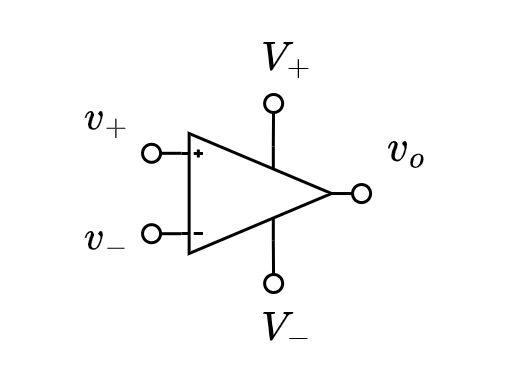
\includegraphics[width=.4\linewidth]{./Images/02Concept/opamp.png}
	\caption{opamp.}
	\label{fig:02opamp}
\end{figure}

\begin{equation}
    v^0 = A(v^+ - v^-)
    \label{eq:simplifiedv^o}
\end{equation}

$V^+$ og $V^-$ er i dette tilfelle spenningsforsyningen, dette setter også begrensningen for opampen da utgangssignalet $v^o$ vil alltid være $V^- < v_o < V^+$.

Fra seksjon \ref{sec:issue} får man oppgitt av en idell opamp har en uendelig stor inngangsmotstand og en utgangsmotstand tilnermet 0. Dette gjør at opampen ikke skal påvirke delsisytemer som den er koblet til. 

En idé til en slik krets kan være en differentialforsterker som vist i figur \ref{fig:differentialforsterker}

\begin{figure}[!hbt]
	\centering
	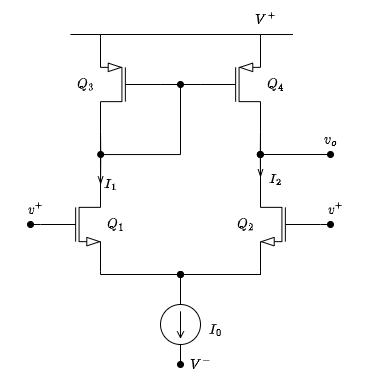
\includegraphics[width=.4\linewidth]{./Images/02Concept/differentialforsterker.png}
	\caption{Differentialforsterker.}
	\label{fig:differentialforsterker}
\end{figure}

Transistorene $Q_{1}$ og $Q_{2}$ er av typen NMOS mens $Q_{3}$ og $Q_{4}$ er av typen PMOS. Disse har en karakteristikk tilsvarende figur \ref{fig:karakteristikkting}.

\begin{figure}[!hbt]
	\centering
	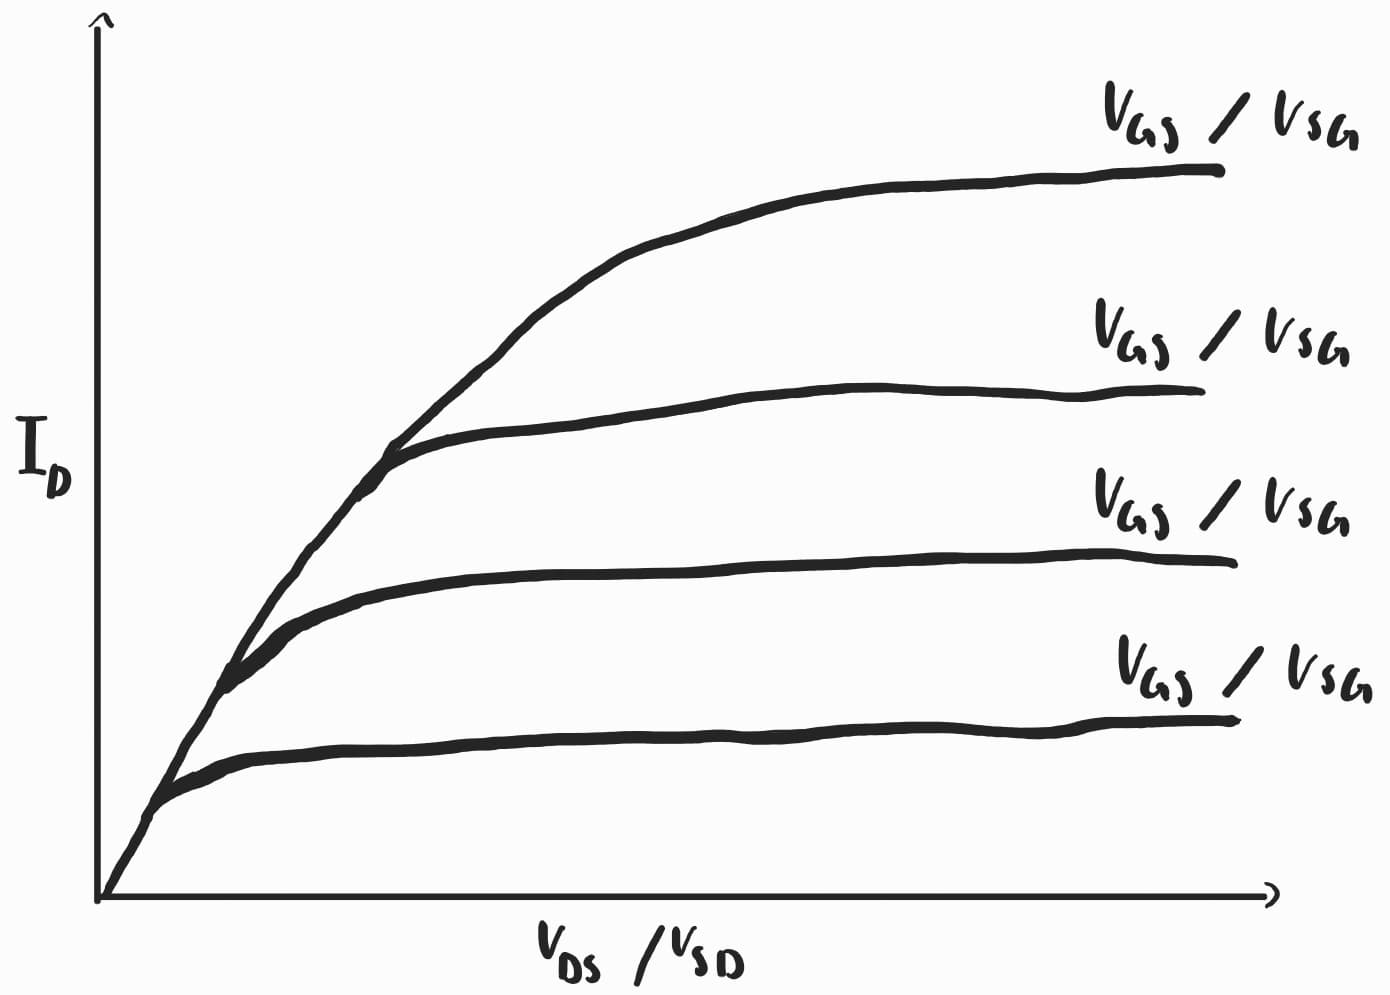
\includegraphics[scale=0.2]{./Images/02Concept/karakteristikkting.jpg}
	\caption{Skisse av karakteristikk ved en MOSFET transistor.}
	\label{fig:karakteristikkting}
\end{figure}

Fra video \cite{feyling_2022_aktiv} opplyses det man at dersom en setter transistorene $Q_3$ og $Q_4$ til å opererer i det aktive området, altså områdene på figur \ref{fig:02karakteristikk} hvor det er mest lineært, Så vil de ha en liten storsignal motstand og samtidig en stor småsignalmotstand. Dermed kan det gå en relativt stor strøm over transistoren uten at spenningsfallet blir noe serlig stort, men samtidig hvis det påtrykkes et lite småsingnal på inngangen slik at strømmen igjennom transistoren får et lite småsignal variasjon, så vil dette føre til en stor spenningsvariasjon på utgangen $v_o$

For å kunne holde $Q_3$ og $Q_4$ i det akrive området uten å måtte manuelt justere på gate spenningen så gatene til noden mellom $Q_1$ og $Q_3$ som vist i figur \ref{fig:differentialforsterker}. Dette fører dermed til en negativ tilbakekobling som gjør at spenningsnivået til gatene til $Q_3$ og $Q_4$ alltid vil justere seg til riktig nivå.

For å oppnå en lav utgangsmotstand skriver en  av administratorene i all about electronics \cite{admin_2021_mosfet} at kan man legge til en source-følger av typen vist i figur \ref{fig:source} på utgangssignalet.

\begin{figure}[!hbt]
	\centering
	\includegraphics[scale=0.5]{./Images/02Concept/source_følger.drawio.png}
	\caption{Source følger.}
	\label{fig:source}
\end{figure}

Strømkilden fra figur \ref{fig:differentialforsterker} kan lages som vist i figur \ref{fig:strømkilde}

\begin{figure}[!hbt]
	\centering
	\includegraphics[scale=0.5]{./Images/02Concept/strømkilde.png}
	\caption{Strømkilde.}
	\label{fig:strømkilde}
\end{figure}

Her brukes potensiometeret $R_P$ til å justere gate-spenningen slik at man kan få et nokså konstant strøm som kan styres. 

Hele systemens kretsdiagram er vist i figur

\begin{figure}[!hbt]
	\centering
	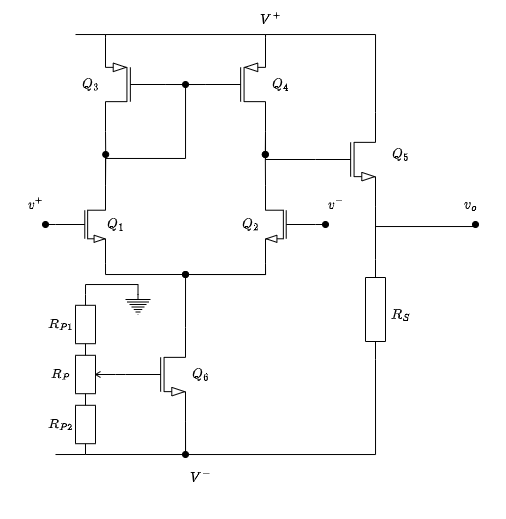
\includegraphics[scale=0.7]{./Images/02Concept/full_kretes.drawio.png}
	\caption{Hele systemets kretsdiagram.}
	\label{fig:kretsdiagram}
\end{figure}